\documentclass{beamer}
\mode<presentation>
\usepackage{amsmath}
\usepackage{amssymb}
%\usepackage{advdate}
\usepackage{adjustbox}
\usepackage{subcaption}
\usepackage{enumitem}
\usepackage{multicol}
\usepackage{mathtools}
\usepackage{listings}
\usepackage{url}
\def\UrlBreaks{\do\/\do-}
\usetheme{Boadilla}
\usecolortheme{lily}
\setbeamertemplate{footline}{
  \leavevmode%
  \hbox{%
    \begin{beamercolorbox}[wd=.9\paperwidth,ht=2.25ex,dp=1ex,left]{author in head/foot}%
      \hspace{1em} Abhijeet Kumar % Your name here
    \end{beamercolorbox}%
    \begin{beamercolorbox}[wd=.1\paperwidth,ht=2.25ex,dp=1ex,right]{author in head/foot}%
      \insertframenumber{} / \inserttotalframenumber\hspace*{2ex}
    \end{beamercolorbox}}%
}
\setbeamertemplate{navigation symbols}{}
\newcommand{\degree}{^{\circ}}
\providecommand{\nCr}[2]{\,^{#1}C_{#2}} % nCr
\providecommand{\nPr}[2]{\,^{#1}P_{#2}} % nPr
\providecommand{\mbf}{\mathbf}
\providecommand{\pr}[1]{\ensuremath{\Pr\left(#1\right)}}
\providecommand{\qfunc}[1]{\ensuremath{Q\left(#1\right)}}
\providecommand{\sbrak}[1]{\ensuremath{{}\left[#1\right]}}
\providecommand{\lsbrak}[1]{\ensuremath{{}\left[#1\right.}}
\providecommand{\rsbrak}[1]{\ensuremath{{}\left.#1\right]}}
\providecommand{\brak}[1]{\ensuremath{\left(#1\right)}}
\providecommand{\lbrak}[1]{\ensuremath{\left(#1\right.}}
\providecommand{\rbrak}[1]{\ensuremath{\left.#1\right)}}
\providecommand{\cbrak}[1]{\ensuremath{\left\{#1\right\}}}
\providecommand{\lcbrak}[1]{\ensuremath{\left\{#1\right.}}
\providecommand{\rcbrak}[1]{\ensuremath{\left.#1\right\}}}
\theoremstyle{remark}
\newtheorem{rem}{Remark}
\newcommand{\sgn}{\mathop{\mathrm{sgn}}}
\providecommand{\abs}[1]{\left\vert#1\right\vert}
\providecommand{\res}[1]{\Res\displaylimits_{#1}} 
\providecommand{\norm}[1]{\lVert#1\rVert}
\providecommand{\mtx}[1]{\mathbf{#1}}
\providecommand{\mean}[1]{E\left[ #1 \right]}
\providecommand{\fourier}{\overset{\mathcal{F}}{ \rightleftharpoons}}
%\providecommand{\hilbert}{\overset{\mathcal{H}}{ \rightleftharpoons}}
\providecommand{\system}{\overset{\mathcal{H}}{ \longleftrightarrow}}
	%\newcommand{\solution}[2]{\textbf{Solution:}{#1}}
%\newcommand{\solution}{\noindent \textbf{Solution: }}
\providecommand{\dec}[2]{\ensuremath{\overset{#1}{\underset{#2}{\gtrless}}}}
\newcommand{\myvec}[1]{\ensuremath{\begin{pmatrix}#1\end{pmatrix}}}
\let\vec\mathbf

\lstset{
%language=C,
frame=single, 
breaklines=true,
columns=fullflexible
}

\numberwithin{equation}{section}
\title{Matgeo 1-1.11-16}
\author{AI24BTECH11001 - Abhijeet Kumar}
\date{\today} 

\begin{document}

\begin{frame}
\titlepage
\end{frame}

\section*{Outline}
\begin{frame}
\tableofcontents
\end{frame}

\section{Question}
\begin{frame}
\frametitle{Question}

The cartesian equation of a line $AB$ is $\frac{2x-1}{12}=\frac{y+2}{2}=\frac{z-3}{3}$.Find the direction cosines of a line parallel to line $AB$.
\end{frame}

\section{Solution}
\subsection{Terms Used}
\begin{frame}
\frametitle{Terms Used}
\begin{table}[htbp]
    \centering
    \caption{Terms used}
    \label{tab:parameters}
    \begin{tabular}{|p{1.7cm}|p{4cm}|}
    \hline\textbf{Term} & \textbf{Description}\\
    \hline
    $m$&Direction vector of line \\
    \hline
    \end{tabular}
\end{table}
\end{frame}

\subsection{Solution}
\begin{frame}
\frametitle{Solution}

The direction vector of the given line is$\colon$
\begin{equation*}
    \vec{m}=\begin{pmatrix}
        6\\
        2\\
        3
    \end{pmatrix}
\end{equation*}
The unit vector of a line having direction vector $m$ is given by $\colon$
\begin{equation}
    = \frac{m}{||m||}
\end{equation}
The direction cosines are elements of above vector  
\end{frame}

\begin{frame}
\frametitle{Solution}

From 1 the unit vector along $AB$ is$\colon$\\
\begin{equation}
= \frac{1}{\sqrt{49}}\begin{pmatrix}
    6\\
    2\\
    3
\end{pmatrix}
\end{equation}
$\therefore$ The direction cosines of line parallel to line $AB$ are the elements of above vector.
\end{frame}

\subsection{Plot}
\begin{frame}
\frametitle{Plot}
    \begin{center}
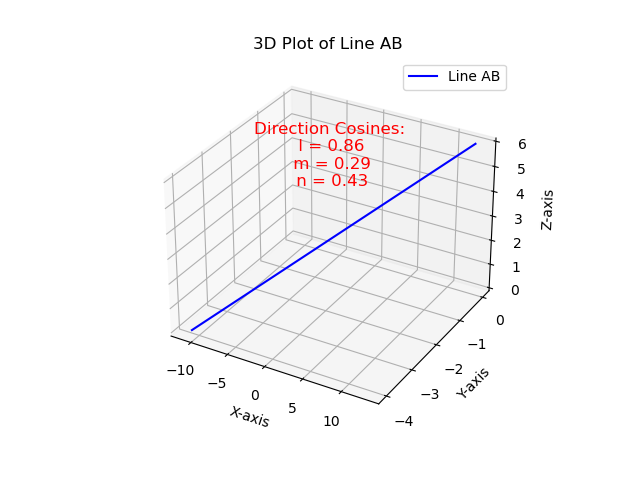
\includegraphics[width=0.9\textwidth]{figs/figure1.png}
\end{center}
\end{frame}

\subsection{C Code}
\begin{frame}
\frametitle{C Code}
    \begin{center}
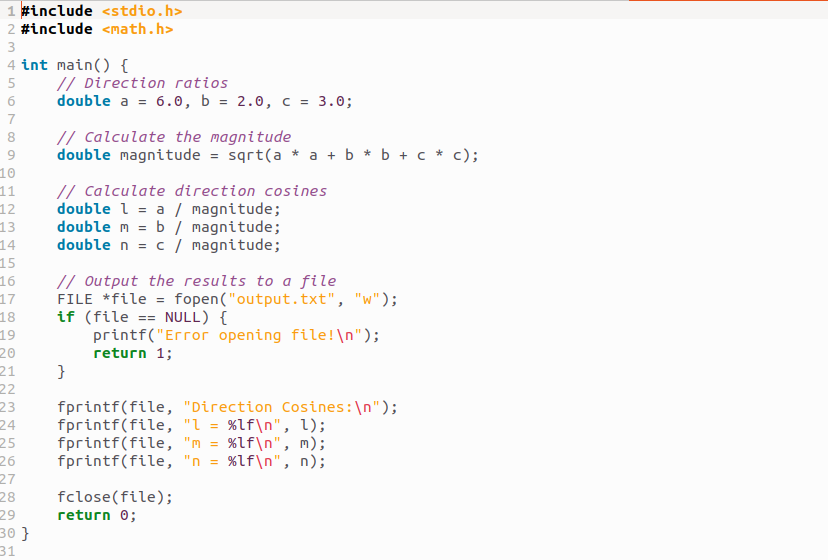
\includegraphics[width=1\textwidth]{figs/figure2.png}
\end{center}
\end{frame}

\subsection{Python Code}
\begin{frame}
\frametitle{Python Code}
    \begin{center}
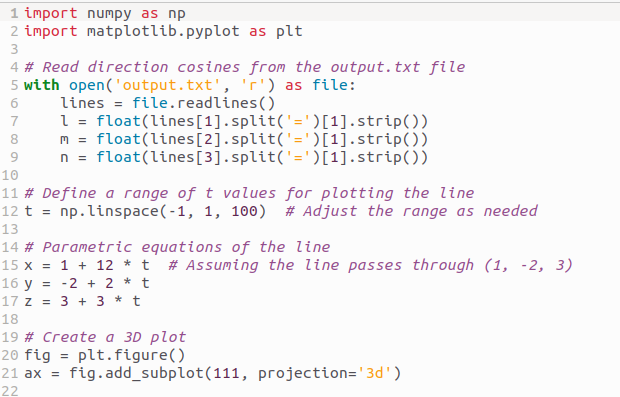
\includegraphics[width=1\textwidth]{figs/figure3.png}
\end{center}
\end{frame}

\begin{frame}
\frametitle{Python Code}
    \begin{center}
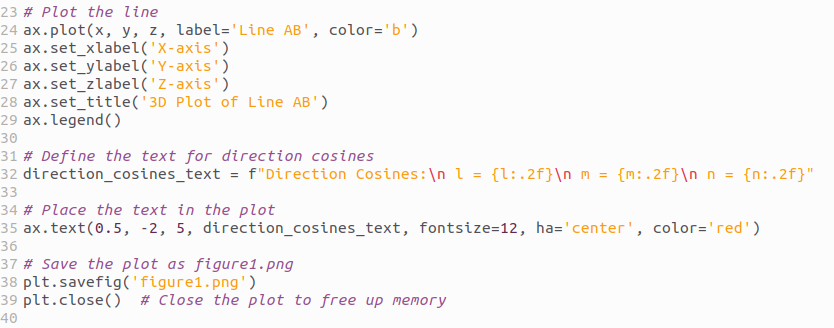
\includegraphics[width=1\textwidth]{figs/figure4.png}
\end{center}
\end{frame}
\end{document}
